\chapter{Luca-Process}
	
Este capitulo describe el proceso de desarrollo e integración del componente gráfico \emph{Process-Component}. Se analizarán los aspectos del diseño y arquitectura a realizar así como las etapas de desarrollo del mismo.
	

El proyecto estará basado en una arquitectura en tres capas. La capa de servicios se comunicará con la capa de repositorio y con una serie de conectores que actuarán de intermediarios con recursos externos al sistema. Además, la capa de presentación utilizará el proyecto implementado con \emph{GoJS} como componente integrado en la interfaz (Figura~\ref{fig:arquitecturaLuca}).

\begin{figure}[H]
	\centering
	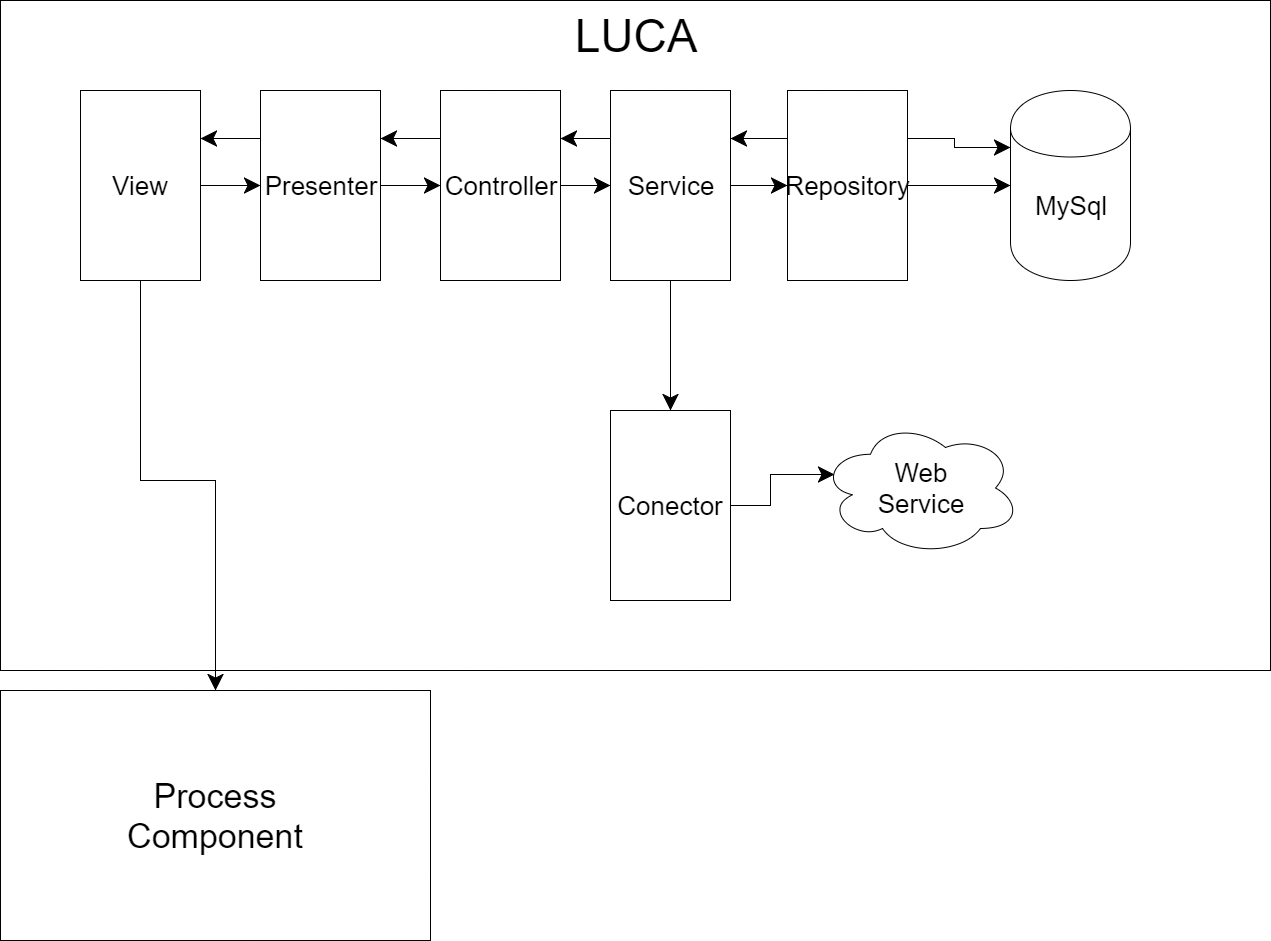
\includegraphics[width=\linewidth]{arquitecturaLuca.png}
	\caption{Nueva Arquitectura de LUCA}\label{fig:arquitecturaLuca}
\end{figure}


El primer paso para empezar a comprender el diseño y arquitectura de LUCA, es entender el patrón MVP\cite{mvp} utilizado.
A nivel de síntesis, el patrón MVP(\emph{Model View Presenter}) consta de tres capas. La capa del \emph{Modelo} es la encargada de albergar toda la lógica de negocio. La capa de la \emph{Vista} posee la capacidad de mostrar datos sobre las diferentes vistas. Por último, la capa de \emph{Presentación} realiza las labores de capa intermedia entre las citadas anteriormente y es capaz de conectar la interfaz gráfica con los daos.


Entrando en el territorio propio de las capas, \emph{LUCA} se compone de tres capas bien diferenciadas:

\begin{enumerate}
	\item Capa de Presentación \subitem Esta capa es la encargada de mostrar los datos sobre la interfaz.
	\item Capa de Servicio \subitem Esta capa se ocupa de obtener los deatos de las diversas fuentes o recursos, ya bien sea comunicándose con la capa de repositorio, o con los diversos conectores hacia fuentes de datos externas. Además, esta capa se divide realmente en dos capas, la mencionada anteriormente, y otra por encima llamada \emph{Controladora} que controla todos los aspectos derivados de la seguridad en el acceso a datos.
	\item Capa de repositorio \subitem Esta capa es la encargada de comunicarse con la base de datos, asi como, de implementar entre otras funciones, los filtros de petición de datos (un ejemplo de filtro sería obtener los datos de los procesos que se encuentren en un estado determinado). Además, se implementa con \emph{Spring Data}\cite{jpa}, que se encarga de asegurar la correcta comunicación con la base de datos.
\end{enumerate}


\section{Pruebas}

La capa de servicio se compone también de un conjunto de pruebas para asegurar su funcionamiento. Sobre la capa de repositorio no es necesario realizar pruebas ya que \emph{Spring Data} asegura su integridad y funcionamiento. Sin embargo, sobre la capa de presentación no se realizaron pruebas automatizadas debido a su complejidad y a que era necesario ajustarse a las fechas de entrega del proyecto.

Las pruebas implementaron y ejecutaron sobre una base de datos en local. Para ello, cada test se compone de un script SQL para introducir los datos previos al test que serán necesarios, y después se ejecuta el test, comprobando mediante \emph{JUnit}\cite{junit} que los resultados son los adecuados.


